\documentclass[12pt]{article}
\usepackage{fontspec}

\setmainfont{Times New Roman} % Times New Roman, Arial, Calibri

\usepackage{setspace}
\setstretch{1.15}


\usepackage{graphicx}
\usepackage{float}

%\usepackage[backend=biber, style=authoryear]{biblatex}
\usepackage[backend=biber, style=numeric]{biblatex}
\addbibresource{references.bib}

\usepackage{geometry}
\geometry{top=2.5cm, bottom=2.5cm, left=2.5cm, right=2.5cm}

\usepackage{pdfpages}

\usepackage{listings}
\usepackage{xcolor}
% Define colors
\definecolor{codegreen}{rgb}{0,0.6,0}
\definecolor{codegray}{rgb}{0.5,0.5,0.5}
\definecolor{codepurple}{rgb}{0.58,0,0.82}
\definecolor{backcolour}{rgb}{0.95,0.95,0.92}

% Setup the listings package
\lstdefinestyle{mystyle}{
    backgroundcolor=\color{backcolour},
    commentstyle=\color{codegreen},
    keywordstyle=\color{magenta},
    numberstyle=\tiny\color{codegray},
    stringstyle=\color{codepurple},
    basicstyle=\ttfamily\footnotesize,
    breakatwhitespace=false,
    breaklines=true,
    captionpos=b,
    keepspaces=true,
    numbers=left,
    numbersep=5pt,
    showspaces=false,
    showstringspaces=false,
    showtabs=false,
    tabsize=2
}

\lstset{style=mystyle}

\title{Identifying Dynamic Systems with Probabilistic Numerics}
\author{Harvey Walton}
\date{\today}

%Repeated Text
\newcommand{\ndiFigCaption}[1]{The rectangle method for finding the #1 bound of the integral of the standard Gaussian (normal) distribution between -2 and 1.}


\begin{document}
    \pagenumbering{roman}

    \thispagestyle{empty}
    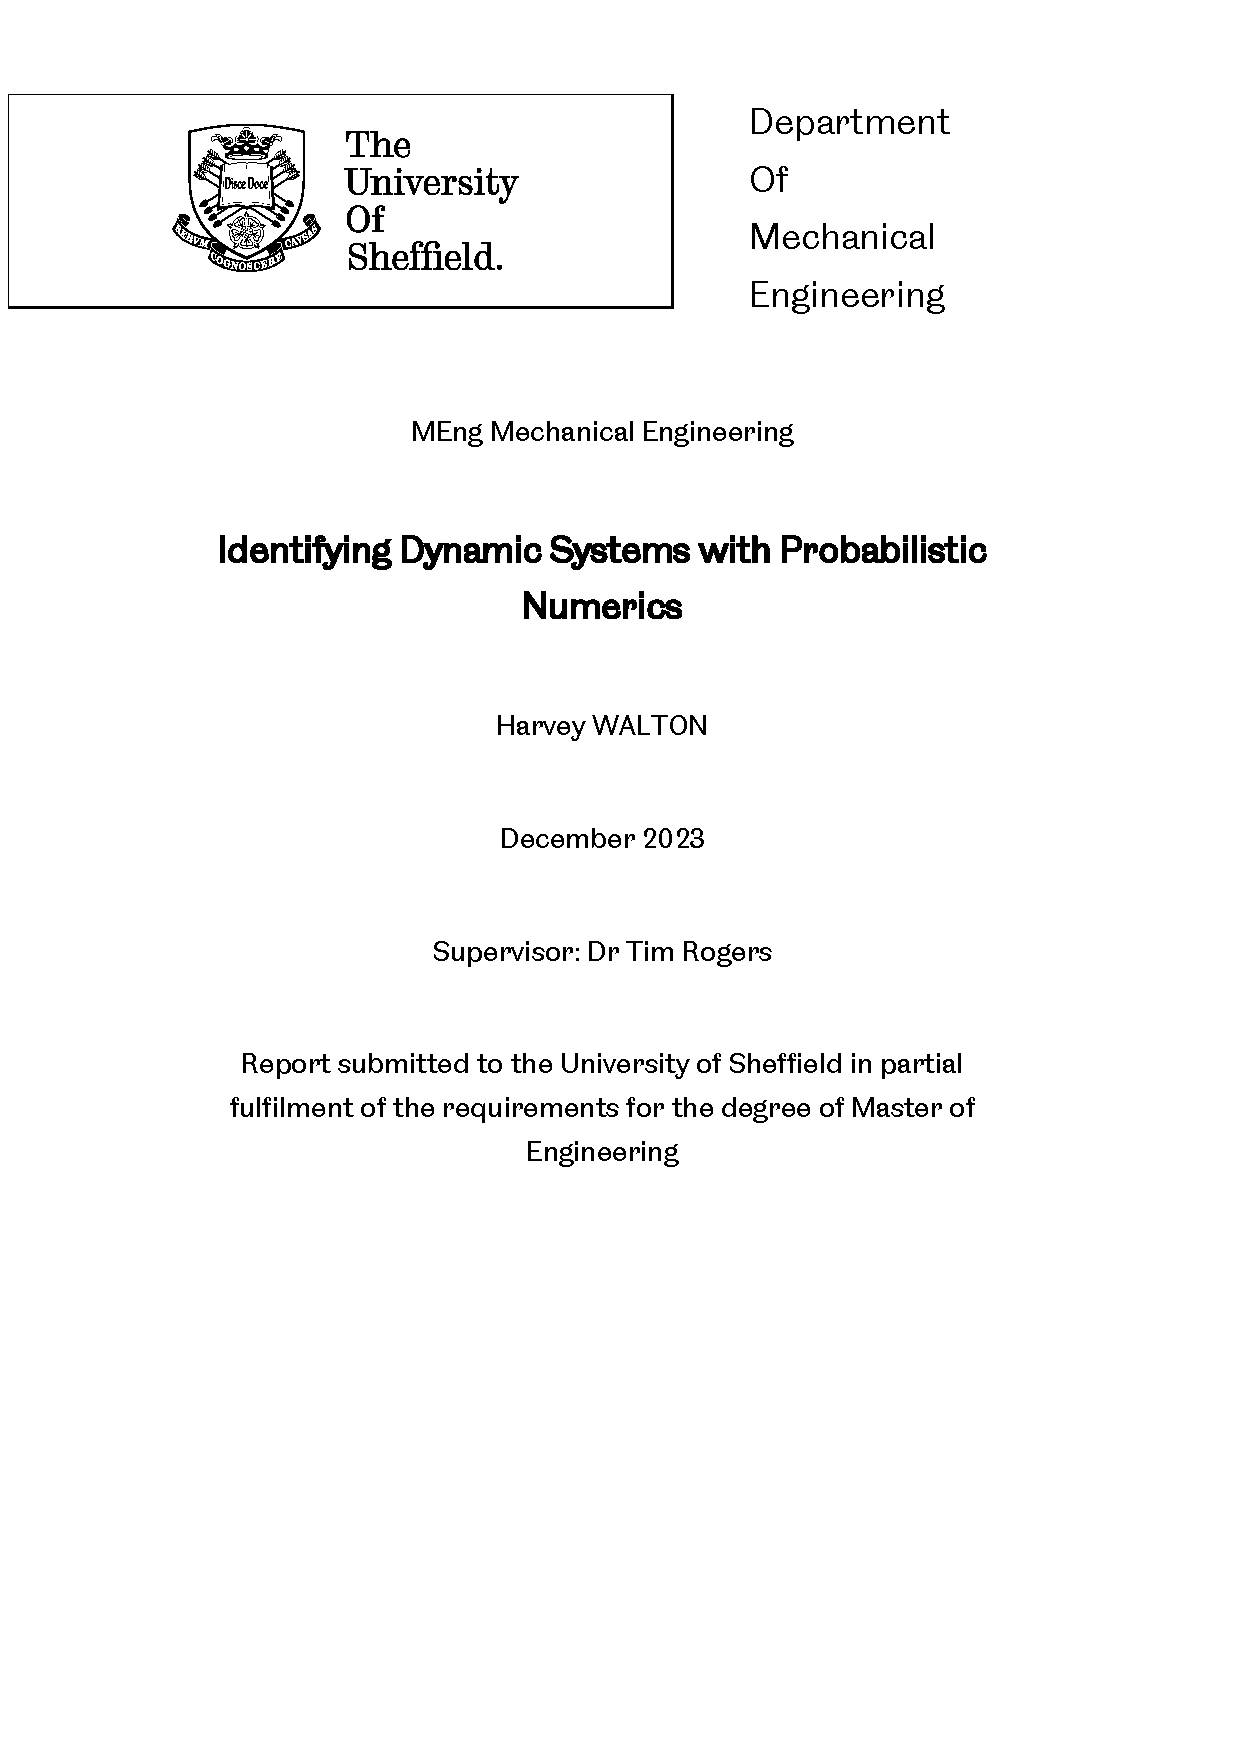
\includepdf[pages=1, frame, scale=1.09, pagecommand={}, offset=0 -35]{figures/titlepage.pdf}


    \tableofcontents
    \newpage

    \pagenumbering{arabic}

    \section{Background and Understanding of the Problem}


    Problems in engineering are usually described using a framework of continuous mathematical functions.
    This means that their output has no jumps or gaps in values, and they can be evaluated using input values that are on a sliding scale of a continuous input domain.
    For example, time in the real world is on a continuous sliding scale, which means that any interval in time can always be subdivided into a smaller interval.
    Continuous functions in turn can often be manipulated analytically using mathematics.
    For example, if the velocity of a particle is given as a continuous function of time, a continuous acceleration function can be derived from the velocity analytically through a mathematical process called differentiation.

    However, there are many situations where this analytical approach is unsuitable:

    \subsection{Intractable Complexity}

    The first reason for this is that the analytical approach may be too complex for anyone to solve.
    A good example of this is the Gaussian (normal) distribution\cite{NIST2023} (Equation~\ref{eq:norm}).

    \begin{equation}
        f(x) = \frac{1}{\sigma\sqrt{2\pi}} \exp\left(-\frac{(x - \mu)^2}{2\sigma^2}\right)\label{eq:norm}
    \end{equation}

    This definite integral of this is often needed in order to find cumulative probabilities (i.e., the chances of a continuous random variable being in a range defined by two values).
    This process can be visualised as finding the area underneath the curve between 2 input values (Figure~\ref{fig:ndi_}).

    \begin{figure}[H]
        \centering
        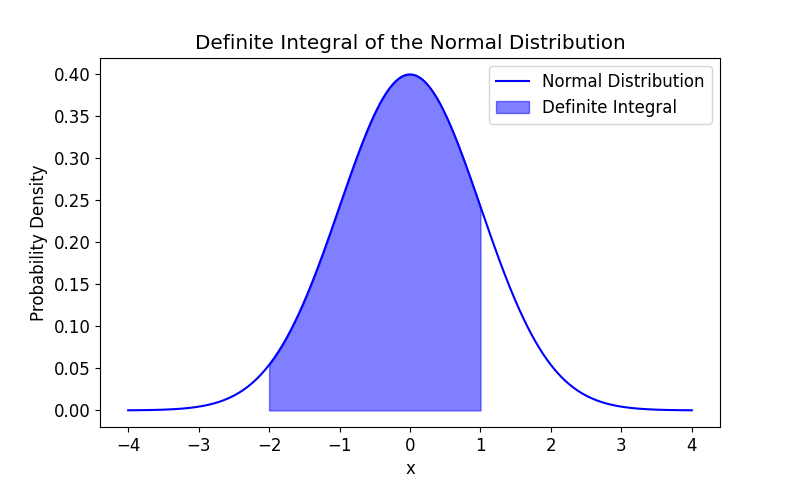
\includegraphics[width=0.8\linewidth]{figures/ndi/ndi_}
        \caption{A definite integral between -2 and 1 of the standard Gaussian (normal) distribution. This is used to find cululative probabilities.}
        \label{fig:ndi_}
    \end{figure}

    In this case, a numerical method is typically used instead such as the Rectangle Method, which uses the Riemann integral definition.
    This states that an integral can be approximated by summing the area of many adjacent rectangles between the function and the axis~\cite{NumericalAnalysis2023}, as shown in Figure~\ref{fig:ndi-num_} and Figure~\ref{fig:ndi-num2_}.

    \begin{figure}[H]
        \centering
        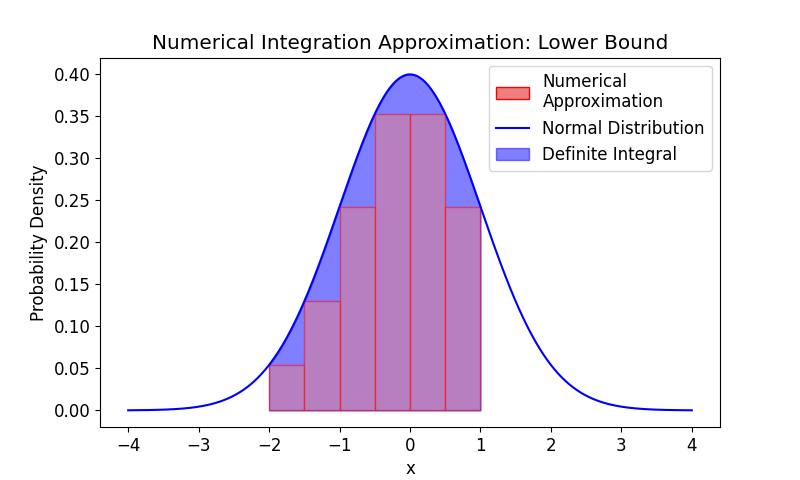
\includegraphics[width=0.8\linewidth]{figures/ndi-num/ndi-num_}
        \caption{\ndiFigCaption{lower}}
        \label{fig:ndi-num_}
    \end{figure}

    \begin{figure}[H]
        \centering
        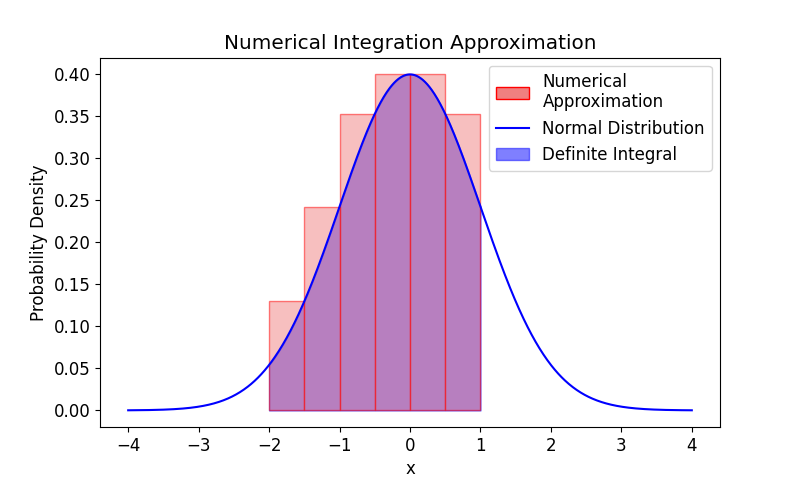
\includegraphics[width=0.8\linewidth]{figures/ndi-num2/ndi-num2_}
        \caption{\ndiFigCaption{upper}}
        \label{fig:ndi-num2_}
    \end{figure}
    As the width of the rectangles approaches zero, the approximation increasingly converges to the exact value of the integral.
    This can never happen in practice, however, because it would require infinite computational work.
    However, we can get good
    As you can see, there are two ways to draw the rectangles.
    In the first method, the top corner of the two that touches the curve is chosen such that the top edge is below the curve.
    This provides an underestimate, which we can use as a lower bound to the true value of the integral.
    Whereas in the second method, the top corner of the two that touches the curve is chosen such that the top edge is above the curve.
    This provides an overestimate, which we can use as an upper bound to the true value of the integral.
    Classically, the quality of this numerical method is computed using the ``error bounds`` ie range between these upper and lower values.

    \subsection{Practical Limits of Data Sampling}
    The second reason is that in practice, the real world continuous data must be sampled at a number of individual points in time.
    A simple example of this is how a video camera discretises the continuous events of the world into individual frames (or ``samples``) that can be replayed back-to-back to recreate an approximation of the events.
    As the frame rate increases, the events are captured in more detail, but the amount of information required to store the approximation tends to infinity and the length of time between frames tends to zero.
    Sampling continuous data in this way discretises the data, which means that analytical mathematical methods that rely on the data being continuous cannot be implemented.
    Again, there are numerical methods that are commonly used to approximate this.
    For example, differentiation is the process of finding the gradient of a continuous function at any location along the curve.
    For a discrete function, the gradient at any point is undefined because you cannot have a tangent of a point.
    However, it is possible to approximate the gradient of the underlying continuous function from which the data was sampled using a numerical method.




    However, to collect data for real world events, it must be sampled or else the amount of information needed to represent the event, as well as the amount of computing power to perform analysis on the event, would tend to infinity.
    Similarly, many problems in the real world are too complex to be solved analytically and so numerical methods are used to approximate the solution to these problems.
    However, what if there was a better approach?
    What if instead of resorting to numerical methods to solve the problem discretely, the original continous data could be reconstructed in ``closed form``.

        However, these methods are not perfect, and introduce error into the solutions.
        This error can be quantified, and is often done so using error bounds


    However, instead, what if the error was quantified using a probability distribution

    Instead, what if we use uncertainty define a pdf of result using (mean and standard deviation)
    in this case, it may be easier to quantify concepts like risk and improve automation of decision-making within engineering
    \subsection{}

    \section{Aims and Objectives}
    Your text goes here.

    \section{Work completed to date}
    Your text goes here. \cite{q-candela}
    \section{Plan for future work}
    Your text goes here.

    \appendix
    \section{The use of generative AI (ChatGPT)}
    OpenAI's ChatGPT interface, powered by the GPT-4 large language model, was used to create some code.
    \subsection{\_inverse\_triangluar\_matrix\ method}
    This method is used to calculate the inverse of R in my method that computes the NLML in my FITC sparse GP approximation.
    It was generated using ChatGPT using the prompt: ``Write a Python function named \_inverse\_upper\_triangular that calculates the inverse of an upper triangular matrix in a faster and more numerically stable way than the standard np.linalg.inv function``.
    The output is provided in Figure~\ref{fig:chat-iut}.:
    \begin{figure}[H]
        \centering
        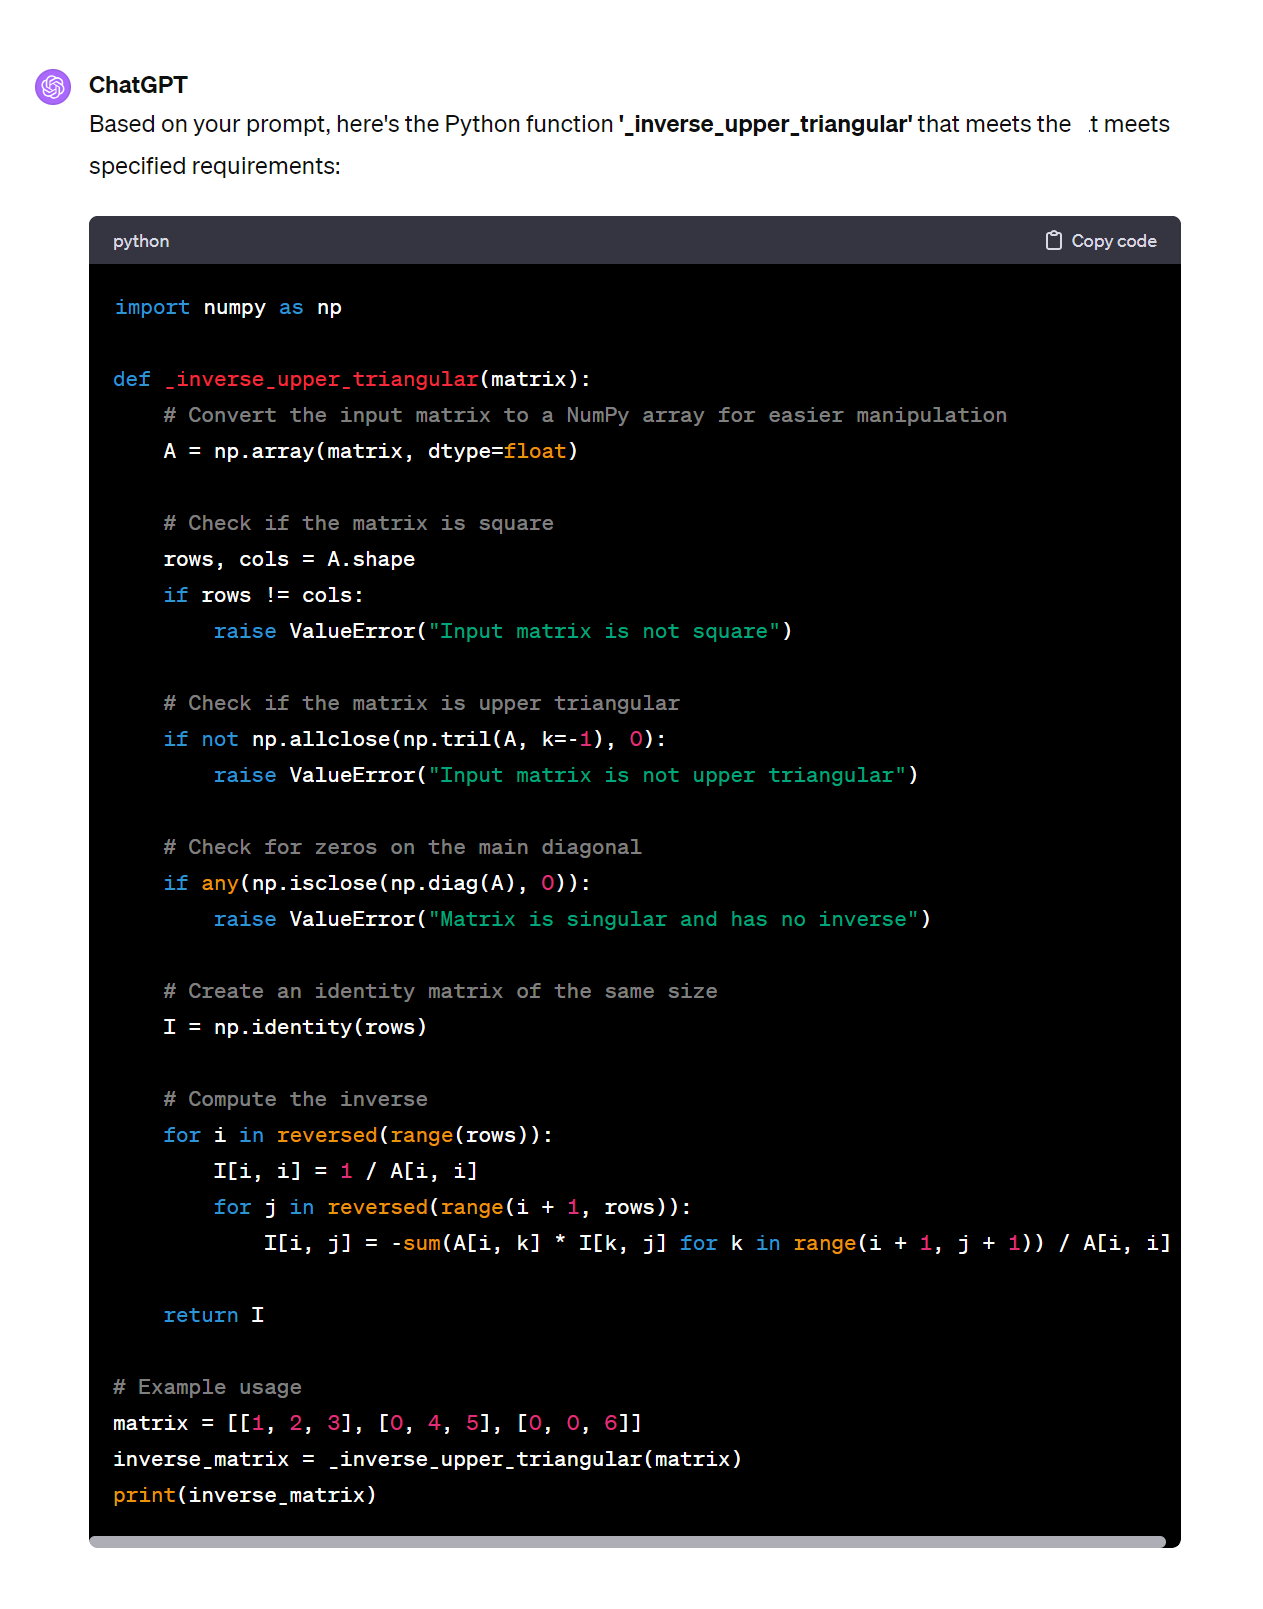
\includegraphics[width=1.1\linewidth]{figures/chat-iut/chat-iut.png}
        \caption{ChatGPT output providing a function used to inverse an upper triangular matrix in a faster and more numerically stable way}
        \label{fig:chat-iut}
    \end{figure}

    After this was generated, it was modified slightly to make it work in my FITC class.
    Firstly, it was made a method instead of a function by adding ``self`` to the inputs.
    Secondly, the output was transformed into a np.array type which is expected for the subsequent code.
    The resulting method is provided below:
    \begin{lstlisting}[language=Python]
    def _inverse_upper_triangular(self, matrix):
        # Convert the input matrix to a NumPy array for easier manipulation
        A = np.array(matrix, dtype=float)

        # Check if the matrix is square
        rows, cols = A.shape
        if rows != cols:
            raise ValueError("Input matrix is not square")

        # Check if the matrix is upper triangular
        if not np.allclose(np.tril(A, k=-1), 0):
            raise ValueError("Input matrix is not upper triangular")

        # Check for zeros on the main diagonal
        if any(np.isclose(np.diag(A), 0)):
            raise ValueError(
                "Matrix is singular and has no inverse")  # Changed from return None for consistency

        # Create an identity matrix of the same size
        I = np.identity(rows)

        # Compute the inverse
        for i in reversed(range(rows)):
            I[i, i] = 1 / A[i, i]
            for j in reversed(range(i + 1, rows)):
                I[i, j] = -sum(A[i, k] * I[k, j] for k in range(i + 1, j + 1)) / A[i, i]

        return np.array(I.tolist())
    \end{lstlisting}

    This was proven to work by writing a unit test:

    \begin{lstlisting}[language=Python]
    def test__inverse_upper_triangular(self):
        obj = GP_NLL_FITC(1, 2, 3, 4, 5, 6)

        # Upper triangular matrix
        matrix = np.array([
            [2, 3, 1],
            [0, 4, 5],
            [0, 0, 7]
        ])

        start_time = timer.time()

        result = obj._inverse_upper_triangular(matrix)

        end_time = timer.time()
        elapsed_time = end_time - start_time
        print(f"The _inverse_upper_triangular func ran in {elapsed_time} seconds")

        start_time = timer.time()

        correct = np.linalg.inv(matrix)

        end_time = timer.time()
        elapsed_time = end_time - start_time
        print(f"The np.linalg.inv func ran in {elapsed_time} seconds")

        debug_print(f"result = {result}")
        debug_print(f"correct = {correct}")
        debug_print(f"difference = {result - correct}")

        assert np.allclose(result, correct, atol=1E-5, rtol=1E-5)

        # Another upper triangular matrix with different values
        matrix2 = np.array([
            [-1.9883, 2.0, 3.0],
            [0, -9.4199, 4.0],
            [0, 0, 1.7969]
        ])
        start_time = timer.time()

        result2 = obj._inverse_upper_triangular(matrix2)

        end_time = timer.time()
        elapsed_time = end_time - start_time
        print(f"The _inverse_upper_triangular func ran in {elapsed_time} seconds")

        start_time = timer.time()

        correct2 = np.linalg.inv(matrix2)

        end_time = timer.time()
        elapsed_time = end_time - start_time
        print(f"The np.linalg.inv func ran in {elapsed_time} seconds")

        debug_print(f"result2 = {result2}")
        debug_print(f"correct2 = {correct2}")
        debug_print(f"difference2 = {result2 - correct2}")

        assert np.allclose(result2, correct2, atol=1E-5, rtol=1E-5)
    \end{lstlisting}

    This compared the result calculated by the method with an expected result calculated using the standard \texttt{np.linalg.inv} function for the two different input matrices.
    If they were the same within both a relative and absolute tolerance of $1E-5.$

    The unit test passed, showing that the function inverses the matrix correctly, however, it wasn't necessarily faster than the standard \texttt{np.linalg.inv} function.
    The inverse of the first matrix was calculated in $0.000246$ and $0.001368$ seconds using \texttt{\_inverse\_upper\_triangular} and \texttt{np.linalg.inv} methods respectively, whereas the inverse of the second matrix was calculated in $0.000312$ and $0.00005$ seconds respectively.
    This indicates that the fastest method depends on the input matrix, which is likely true for larger matrices also since both functions are of the $O(n^3)$ for an $n \times n$ matrix.
    However, the \texttt{\_inverse\_upper\_triangular} function will be more numerically stable and memory efficient because it is taking adavantages of the fact that the input matrix is upper triangular which allows the inverse to be found by back substitution instead of it being computed naively.

    \subsection{Figures for the report}
    \subsubsection{Cumulative Distribution Function}
    Put prompt and output


    \printbibliography

\end{document}
